% ----
% COMP1204 CW1 Report Document
% ----
\documentclass[]{article}

% Reduce the margin size, as they're quite big by default
\usepackage[margin=1in]{geometry}

%Importing fancy package
\usepackage{fancyvrb}
\usepackage[most]{tcolorbox}
\usepackage{xcolor}
\usepackage{graphicx}
\graphicspath{ {./images/} }

\title{COMP1204: Data Management \\ Coursework One: Hurricane Monitoring }
% Update these!
\author{Damien Ta \\ 34830294}

% Actually start the report content
\begin{document}

% Add title, author and date info
\maketitle

\section{Introduction}
As data scientists for the National Oceanographic and Atmospheric Administraiton Centre, I was assigned to the tropical cyclone
tracking team. As a data scientist I have been tasked with extracting storm data from the tropical cyclone reports and producing
maps of where the cyclones have taken place.
\section{Create CSV Script}
Here's my script:
\begin{tcolorbox}[colback=white, colframe=black, boxrule=0.5pt, arc=2mm, 
    title=create\_csv.sh, fonttitle=\bfseries, listing only, listing options={language=sh, basicstyle=\ttfamily}]
    \begin{verbatim}
#!/bin/bash
csv_input_path=$1
tmp_csv_output=$2

#I used \ to continue command on next line

echo "Timestamp,Latitude,Longitude,MinSeaLevelPressure,MaxIntensity" > $tmp_csv_output
dtg="$(grep -R "<dtg>" $csv_input_path | sed 's/.*<dtg>//g' | sed 's/[</dtg>]//g')"

grep -R "<lat>" $csv_input_path| sed 's/.*<lat>//g' | sed 's/[</lat>]//g' > lat.csv
grep -R "<lon>" $csv_input_path | sed 's/.*<lon>//g' | sed 's/[</lon>]//g' > lon.csv
grep -R "<minSeaLevelPres>" $csv_input_path | sed 's/.*<minSeaLevelPres>//g' | \
sed 's/[</minSeaLevelPres>]//g' > minSeaLevelPres.csv
grep -R "<intensity>" $csv_input_path | sed 's/.*<intensity>//g' | \ 
sed 's/[</intensity>]//g' > intensity.csv

lat="$(sed "s/$/ N/" lat.csv)"
lon="$(sed "s/$/ W/" lon.csv)"
minSeaLevelPres="$(sed "s/$/ mb/" minSeaLevelPres.csv)"
maxIntensity="$(sed "s/$/ knots/" intensity.csv)"

paste -d',' <(echo "$dtg") <(echo "$lat") <(echo "$lon") <(echo "$minSeaLevelPres") \
<(echo "$maxIntensity") >> $tmp_csv_output
rm lat.csv
rm lon.csv
rm minSeaLevelPres.csv
    \end{verbatim}
\end{tcolorbox}



\section{Storm Plots}
\begin{figure}[htbp]
    \centering
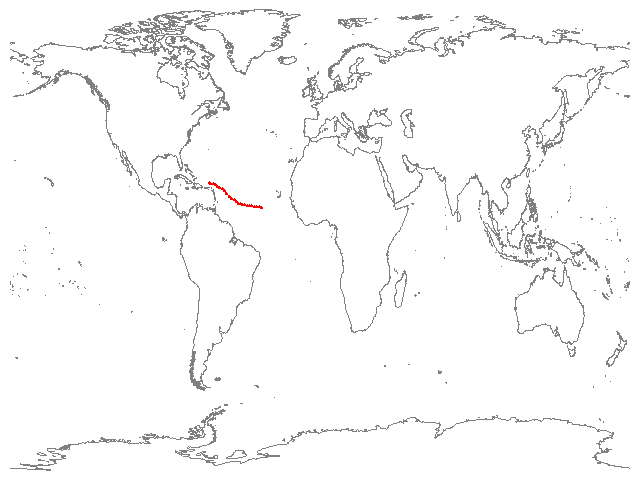
\includegraphics{al112020.png}
\caption{al112020.kml}
\label{fig:al112020}
\end{figure}

\begin{figure}[htbp]
    \centering
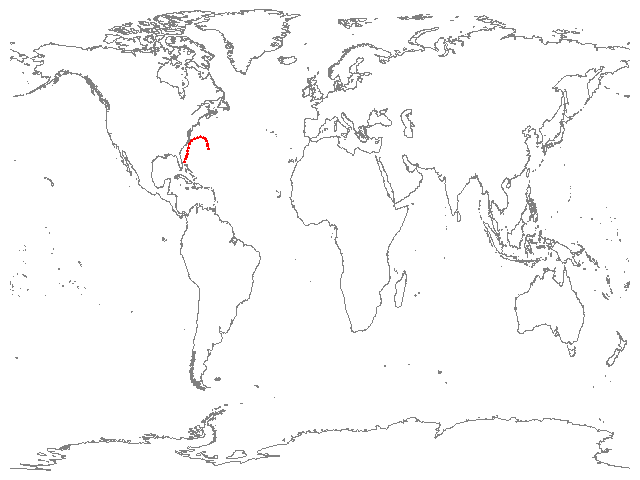
\includegraphics{al012020.png}
\caption{al012020.kml}
\label{fig:al012020}
\end{figure}

\begin{figure}[htbp]
    \centering
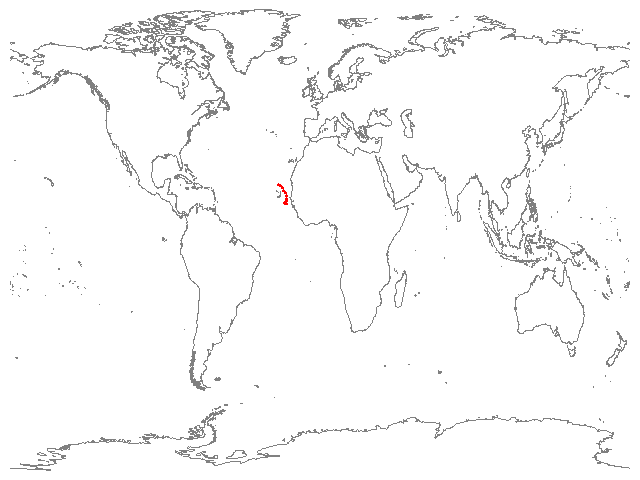
\includegraphics{al102020.png}
\caption{al102020.kml}
\label{fig:al102020}
\end{figure}
\clearpage
\section{Git Usage}
\begin{tcolorbox}[enhanced, 
    listing only,
    title=Python Code for Plotting CSV Data,
    fonttitle=\bfseries,
    colback=white,
    colframe=black!70,
    listing options={
      language=Python,
      numbers=left, 
      numberstyle=\tiny\color{gray},
      breaklines=true, 
      basicstyle=\ttfamily\small, 
      columns=fullflexible,
      keepspaces=true,
      showstringspaces=true,
    },]
    \begin{verbatim}
        import pandas as pd
        import matplotlib.pyplot as plt
        import os
        import glob
        import math
        user_key = 1773
        
        def plot_all_csv_pressure():
            path = os.getcwd()
            csv_files = glob.glob(os.path.join(path, '*.csv'))
            
            for f in csv_files:
                storm = pd.read_csv(f)
                storm['Pressure'].plot()
                plt.show()
        
        def plot_all_csv_intensity():
            path = os.getcwd()
            csv_files = glob.glob(os.path.join(path, '*.csv'))
            
            for f in csv_files:
                storm = pd.read_csv(f)
                storm['Intensity'].plot()
                plt.show()
    \end{verbatim}
\end{tcolorbox}


\end{document}
